%% LyX 2.3.2-2 created this file.  For more info, see http://www.lyx.org/.
%% Do not edit unless you really know what you are doing.
\documentclass[english]{revtex4-1}
\usepackage[T1]{fontenc}
\usepackage[latin9]{inputenc}
\setcounter{secnumdepth}{3}
\usepackage{float}
\usepackage{graphicx}
\usepackage{babel}
\begin{document}
\title{Prelim document draft.}

\maketitle
By making an Al/Na3Bi heterostructure, we can make topological states?

\section{Introduce Topological Insulators and Topological Dirac Semimetals.}

Topological materials have garnered significant attention in the condensed matter community in past few years because of their peculiar electronic properties both in the uncorrelated and strongly correlated materials. Here We will focus on the uncorrelated topological systems. The first relevant system is what is known as a topological insulator. Topological insulators feature a insulating (or gapped band spectrum) in their bulk but are conducting (or gapless) on the surface that encloses the bulk. The gapless states on their surfaces are termed chiral currents, which are characterized by spin-momentum locking. Effectively, the propagation direction of the charge carriers is set by their spin degree of freedom. Moreover, at energies and momenta near the surface band crossing points in these systems, the dispersion attains a form of a non-relativistic version of a massless Dirac dispersion relation. Overall, topological insulators like $BiS3_3$ have a crucial symmetry known as time-reversal symmetry, which prevents the chiral surface states from being gapped.   Initially these peculiar electronic characteristics were thought to exist in graphene.

Since then, new materials which feature both a gapless bulk and surface states have been discovered theoretically and experimentally. These materials are known as topological semimetals. They are grouped into two general types of topological semimetals: Weyl and Dirac semimetals. Part of this classification is based on the type of degeneracies in the band plots. We will provide a short explanation on their differences.

In a band structure plot of the energy states there are cases where
bands corresponding to different energy eigenvalues can be degenerate
from accidental degeneracies (i.e. from tuning parameters in the Hamiltonian such that two or more energy levels can have the same energy). The presence of symmetries can increase the degeneracy of the band crossing points. (There are symmetries that can induce band crossings?) Most of the 3-D semimetals have T.R.S and inversion symmetry. Inversion
symmetry reverses the sign of the momentum, but not the spin of the
particular band: $E_{n,\sigma}\left({\bf k}\right)=E_{n,\sigma}\left(-{\bf k}\right)$. Time reversal symmetry reverses both the spin of the particular band and the sign of the momentum:$E_{n,\uparrow}\left({\bf k}\right)=E_{n,\downarrow}\left(-{\bf k}\right)$.
If both time-reversal symmetry and inversion symmetry are present,
then:$E_{n,\uparrow}\left({\bf k}\right)=E_{n,\downarrow}\left({\bf k}\right)$,
which indicates that there is a double degeneracy for bands of different
spin components at each k-point. If there is a degeneracy of bands,
at some momentum ${\bf k}_{0}$, of different quantum number $n$,
say $n$ and $n+1$, then that band crossing point is four-fold degenerate.
If we expand the Hamiltonian at the band crossing point and if this
gives a massless Dirac dispersion relation, then this band crossing
point can be regarded as an emergent and non-relativistic Dirac particle.
In the case where there is a breaking of time-reversal symmetry, or
inversion-symmetry, or both, the double degeneracy of the a single
band is lifted over generic points in the Brillouin zone. In this
case, when two such bands meet at the same energy at some momentum
in the Brillouin zone, there is a degeneracy of two. If one expands
the Hamiltonian around the momentum crossing point of the two bands,
and if one finds a relativistic Weyl dispersion, such band crossings
are called Weyl nodes. Each Weyl node carries a non-zero ``charge''
which is computed by integrating the Berry curvature around a small
closed surface $S$ that encloses the Weyl node.  This is defined as the Chern number:

\begin{equation}
C = \frac{1}{2\pi} \oint_S \vec{\Omega}_{n}(\vec{k}) \cdot d\vec{S}_{\vec{k}}    
\end{equation}

\section{Some of our data.}

%Baseline system: Na3Bi topological Dirac semimetal.
We decided to look at the topological Dirac semimetal Na3Bi in the
(110) direction. The reason why we chose this direction was because
this surface is parallel to the $k_{z}$ axis along which there are two Dirac point crossings. Therefore, Fermi arc surface states may appear on
this surface for a specific $k_{z}$ value, $k_{z}=0$ to be more
exact since it is a plane that has time-reversal symmetry.

%Na3Bi band gap oscillations.
\subsection{Na3Bi (110) slab and vacuum thickness effects on Na3Bi's band structure.}

\begin{figure}[H]
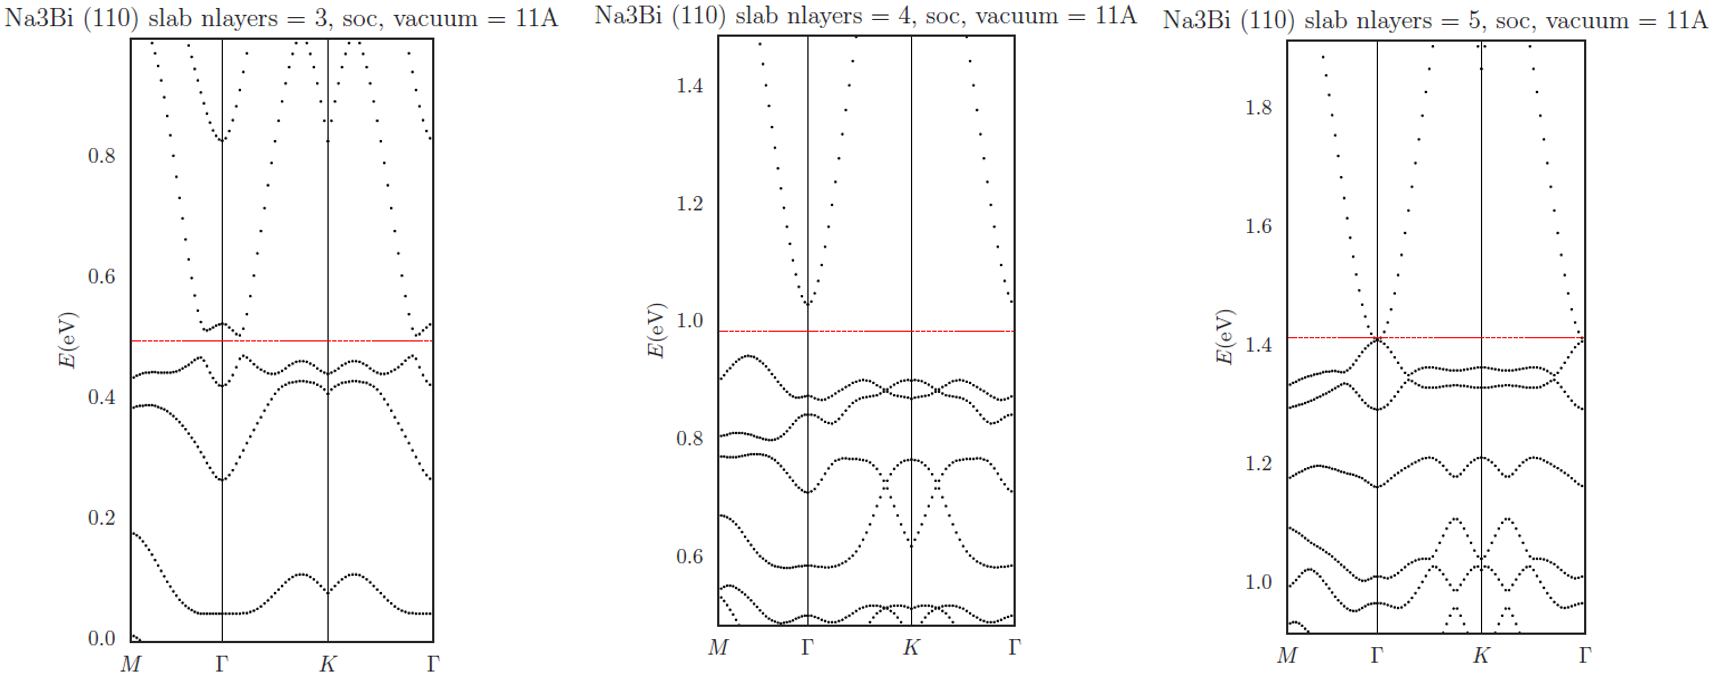
\includegraphics[scale=0.5]{Na3Bi_change_nlayers_vac_11A}\caption{\label{fig:Band-plots-of Na3Bi changing thickness}Band plots of the
Na3Bi (110) system with fixed vacuum thickness but varying system
thickness.}
\end{figure}

We see in Figure \ref{fig:Band-plots-of Na3Bi changing thickness}
the effects of increasing the thickness of Na3Bi on the band structure.
We find an oscillatory behavior in the band gap with larger band gaps
observed for even layers while odd layers give smaller band gaps near
the $\Gamma$ point.  (Cite paper here that mentions the oscillatory behavior of Na3Bi's band gap when the confining direction (i.e. the direction with open boundary conditions) is along the z-direction). 
(Why are we interested in the $\Gamma$ point?
It is perhaps because at that momentum, the band inversion is most
visible. We see hints of the band inversion for the 3 layer Na3Bi
(110) structure above at the $\Gamma$ point, for the conduction and
valence bands nearest the Fermi level.).

\begin{figure}[H]
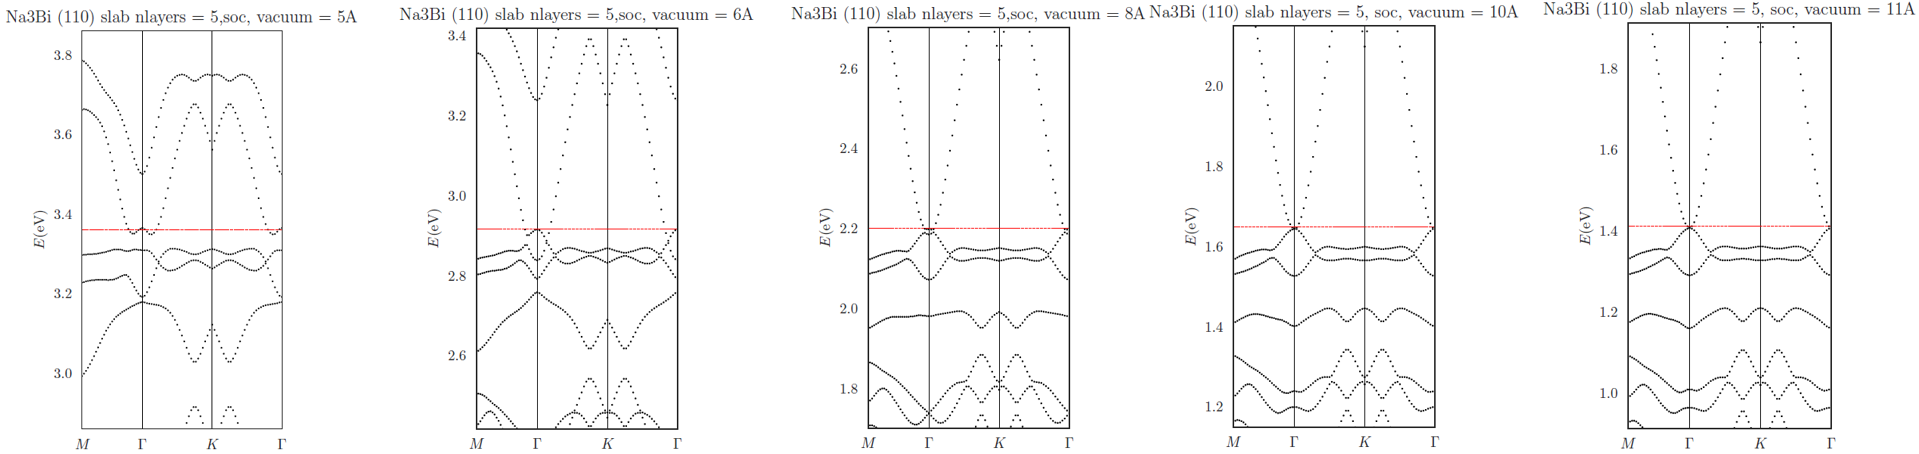
\includegraphics[scale=0.5]{Na3Bi_nlayer_5_change_vac}\caption{\label{fig:Na3Bi Fixed odd number layers incr vac}Fixed odd number
of Na3Bi layers with increasing vacuum thickness.}
\end{figure}

In Figure \ref{fig:Na3Bi Fixed odd number layers incr vac} , we fix
the number of layers in the Na3Bi system to 5, and we adjust the vacuum thickness. We find there are hints of band inversion for the bands nearest the Fermi level at the $\Gamma$ point for the 5 layer Na3Bi system surrounded by an 8A vacuum layer. Overall the band structures demonstrate little to no band gaps in the energies around the Fermi level near the $\Gamma$ point.

\begin{figure}[H]
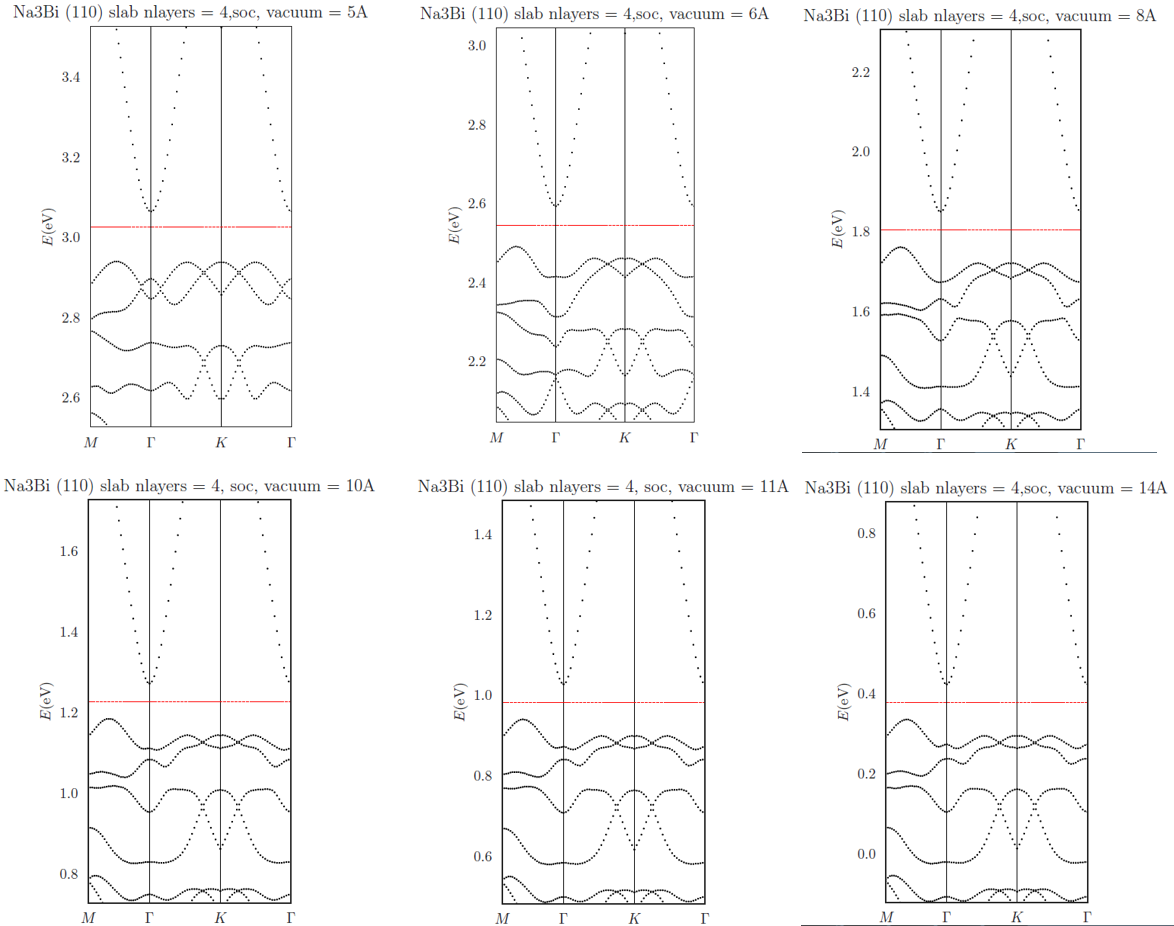
\includegraphics[scale=0.5]{Na3Bi_nlayer4_change_vac}

\caption{\label{fig:Na3Bi Fixed even number layers incr vac}Fixed even number
of Na3Bi layers with changing vacuum thickness.}
\end{figure}

By inspection of Figure \ref{fig:Na3Bi Fixed even number layers incr vac},
we observe a relatively large band gap, compared with the odd number
of layers for Na3Bi. It does not appear that there is band inversion
in the character of the bands nearest to the Fermi level and at the
$\Gamma$ point. Overall, we need to find the Berry curvature of these
systems in order to definitively determine their topological characteristics.

\subsection{Aluminum on Na3Bi heterostructure data.}

We want to investigate the fate of the Na3Bi surface states when Na3Bi
is adjacent to Aluminum (Al). In particular we want to answer whether
there is any hybridization of the Na3Bi surface states with the Al
metallic states, and also to observe how far the spin texture characterizing the Na3Bi surface states penetrate into the Al surface. Since Na3Bi and Al have distinct crystal structures, Na3Bi having a hexagonal P63/mmc phase crystal structure while Al has a face-centered cubic crystal structure, they need to be stacked in such a way as to minimize the lattice mismatch between both structures. Based on information from the materialsproject website, we selected Al(111) on Na3Bi (110) as the combination that minimizes the lattice mismatch.

\begin{figure}[H]

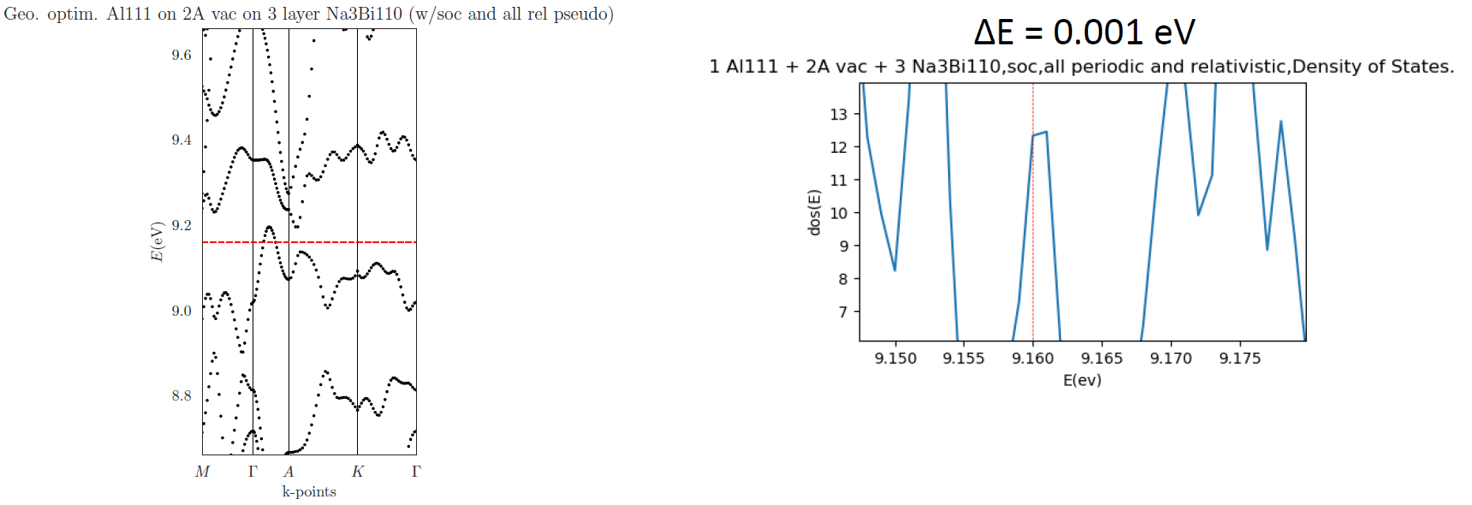
\includegraphics[scale=0.5]{Al111_on_Na3Bi_bandplot&DOS}\caption{\label{fig:1Al+3Na3Bi bandplot =000026 DOS.}Band structure plot and
electronic density of states for geometrically optimized Al/Na3Bi
heterostructure.}

\end{figure}

Up to this point, we have data for an Al/Na3Bi heterostructure which
contains a single layer of Al orientated along the (111) direction
on three layers of Na3Bi orientated along the (110) direction. The
Al layer is separated from the Na3Bi layers by a small spacing of
2A. In Figure \ref{fig:1Al+3Na3Bi bandplot =000026 DOS.}, we see
this heterostructure is metallic since the red dashed line intersects
a band and there is no finite energy gap between the filled and unfilled electronic states. Moreover, we find the same conclusion if we study the density of electronic states. This quantity signifies the number of available electronic states per unit energy per unit volume. We see above that there is a non-zero density of states around the Fermi level. 
\begin{figure}[H]

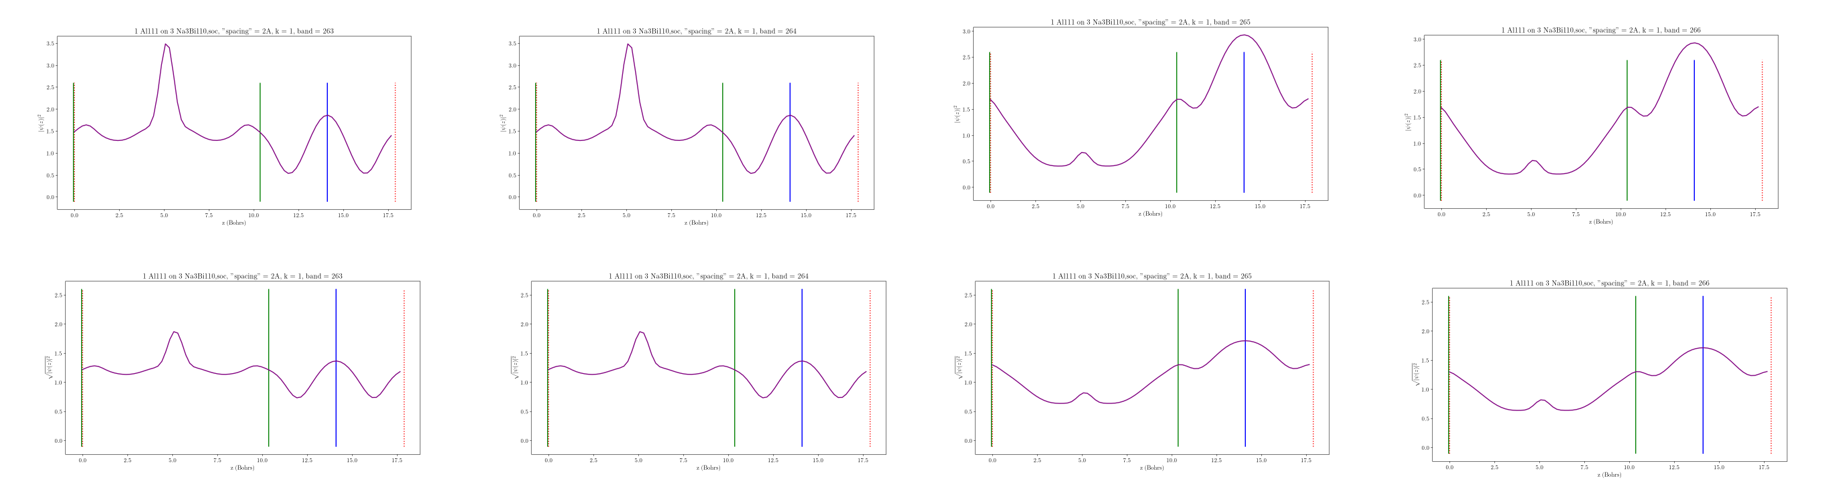
\includegraphics[scale=0.6]{Al111_on_Na3Bi_wavefunctions}\caption{\label{fig:Modulus squared and modulus of bands}Modulus squared and
modulus of bands closest to the Fermi level.}
\end{figure}

In Figure \ref{fig:Modulus squared and modulus of bands} we have
plotted $\left|\psi\left(z\right)\right|^{2}$ and $\sqrt{\left|\psi\left(z\right)\right|^{2}}$of
the bands closest to the Fermi level. The green and blue vertical
lines denote the boundaries of the Na3Bi and Al layers, respectively,
while the red dashed lines are the boundaries of the structure (this
includes any \textquotedblleft vacuum\textquotedblright{} regions).
It appears as though the valence bands (\#263 \& \#264) have a modulus
that is peaked around the center of the Na3Bi system. This modulus
dips in the region between the Na3Bi and Al structure and the Al and
upper structure boundary. There\textquoteright s actually a relative
maximum of the modulus that appears at the Al structure. The conduction
bands (\#265 \& \#266) have a modulus that behaves completely different.
For these bands, their maximum modulus appears around the Al structure.
Other relative maxima occur at the surfaces of the Na3Bi structure.
Between the Na3Bi and Al structure, the modulus is not at all a minimum.
These conduction bands have a minimum around the center of the Na3Bi
structure. As for the analogous square root of the modulus plots,
there\textquoteright s not much to say for them: they appear to follow
the trends of the modulus squared plots. It appears as though these
plots indicate there is no hybridization of the Na3Bi surface states
with the Al states. However, we only have a single Al layer present.
We may want to increase the size of the Al layer. Additionally, we
are attempting to find the behavior of the surface states in a heterostructure consisting of Na3Bi and KTaO3, the latter being an insulator.
\end{document}
